Another challenging program reachability quantitative property is the \emph{non-monotonic} quantitative property.
This kind of property includes memory usage in the presence of garbage collection,
number of channel connections established that is later closed,
or resources requested to a virtual host which is released after using them. 
The non-monotonic quantitative property is significantly different from the traditional monotonic quantitative property,
such as the program execution time, energy consumption,
% etc. w.r.t. the physical resources,
or the information leakage, etc. with different measurements in different areas.
% ).
These traditional quantitative properties only accumulate during the program execution. 
However, the non-monotonic quantitative property could also decrease along the computation.
So it is challenging to give a precise bound via computing the bound on this quantity just for the worst-case or the final execution state in the traditional way.
% And to compute the bound on the quantity.

This section first covers the background of the current research on the non-monotonic
quantitative property analysis in Section~\ref{sec:nonmonotonic-intro}.
Then it introduced the new methodology for analyzing the non-monotonic quantitative property in Section~\ref{sec:nonmonotonic-methodology} with an example demonstrating the methodology.
% % resource cost and quantitative property analysis,
% with a 
% motivating example.
% This example shows that the traditional way fails to give a tight bound on the program's non-monotonic resource cost.
% similarity between general and the program's adaptivity accumulation,
% Then, this section covers the proposed methodology I plan to adopt for an accurate full-Spectrum
% analysis on 
% % the general resource cost analysis.
% the program's resource cost.
\subsection{Introduction }
\label{sec:nonmonotonic-intro}
% Through observation in the following example, the heap resource consumption during the program 
% execution is accumulating in the same way as the program's adaptivity. 
% More specifically in Example~\ref{}Specifically, in line 5 
% where the list is re-written and the heap consumption is decreased implicitly. 
% This implicit decrease 
% of the cost works the same as the program's adaptivity decreases.
% \\
% This motivates the generalization of the analysis framework onto the program's resource cost analysis. Use this framework,
% I will give
% a more accurate resource cost estimation 
% by considering the program's implicit resource cost, comparing 
% to the worst case cost analysis in the traditional way.
% \\
\paragraph*{Non-Monotonic Quantitative Property}

% \paragraph*{Background and Related Work}
Non-cumulative resources are first acquired and then released.
Typical examples are memory usage in the presence of garbage collection, the maximum number of connections established simultaneously, the size of the stack of activation records, etc.
The problem is nowadays also very relevant in virtualized systems, as in cloud computing, 
in which resources are acquired when needed and released after being used.
It is recognized that non-cumulative resources introduce new challenges in resource analysis [5,12].
The challenge incurs when the resource consumption can increase and decrease along the computation, 
and it is not enough to reason only on the final state of the execution in the worst case,
but rather the upper bound on the cost can happen at any intermediate step.

% \todo
{
 In the program quantitative property analysis area, the methodologies are mainly based on
 two different kinds of analysis techniques, type-system-based and the data-flow/control-flow analysis based.
% There are mainly two categories of methodology in the static program resource cost analysis areas, 
% through type-system based and data-flow/control-flow analysis based. 
% They can be summarized as follows but to the best of my knowledge,
% all these works in the two categories fail to recognize the case where program resource consumption is decreased implicitly.
\paragraph*{Type-System Based}
In type-system-based analysis methodology,
they design the effect systems~\cite{cciccek2017relational,radivcek2017monadic,qu2019relational},
Hoare-Logic~\cite{gaboardi2021graded}, or amortized type system~\cite{hoffmann_jost_2022}.
They statically estimate a sound upper bound for the program's cost.
However, they all aim to compute the bound for the traditional resource cost accumulatively
without considering the cost decreasing. 
% Existing
% static program analysis based type-system is mainly through 
% effect systems, 
% % control-flow analysis, and data-flow analysis~\cite{ryder1988incremental}. 
% % The idea of statically estimating a sound upper bound for the adaptivity from the semantics is indirectly inspired by prior 
% Previous work on cost analysis via effect systems~\cite{cciccek2017relational,radivcek2017monadic,qu2019relational} statically estimating a sound upper bound for the program's cost accumulating.
% % The idea of defining adaptivity using data flow is inspired by the work of graded 
% Hoare logic~\cite{gaboardi2021graded}, and amortized type system~\cite{hoffmann_jost_2022}.
% The only way to save the cost on the potential
% type, as 
% The type system in~\cite{GustafssonEL05} and
The amortized type-system designed in \cite{hoffmann_jost_2022} considers a perfect garbage collection
% through explicit abstraction or data structure de-allocation.
% data structure deallocation 
% and they 
estimates the cost decreasing situation by saving the cost into the potential type through destructive pattern match.
However, their language model doesn't have the specific models of garbage collection and they cannot give the 
% That is to say, they cannot deal with the case where the cost (for example the adaptivity) decreases when there isn't a dependency relation between variables.
\paragraph*{Data-flow/Control-flow Analysis Based}
% Existing static program analysis works via 
The control flow or data flow analysis-based methodologies,
% in program resource cost analysis 
% mainly falls into two areas, 
are mainly aimed to estimate the program complexity or worst-case execution time. 
The techniques are based on
% type system~\cite{CicekBG0H17, RajaniG0021}, Hoare logic~\cite{CarbonneauxHS15}, 
abstract interpretation~\cite{GustafssonEL05, HumenbergerJK18},
invariant generation through cost equations or ranking functions~\cite{BrockschmidtEFFG16,AlbertAGP08,AliasDFG10,Flores-MontoyaH14}
or a combination of program abstraction and invariant inferring~\cite{GulwaniZ10, SinnZV17, GulwaniJK09}.
In general, these techniques give the approximated upper bound of the program's total running time or resource cost.
However, they failed to consider the case where the program's cost could decrease when there isn't a dependency relation between variables.
However, they are all focusing on analyzing the traditional accumulative cost of the entire program. 
\\
Some work~\cite{AlbertFR14, BrabermanGHY14, HofmannJ03} in analyzing the memory usage can compute the peak bound specific models of garbage collection,
while they don't give a generic framework to estimate the non-cumulative quantitative property.
\\
The work in \cite{AlbertFR15} gave a generic resource analysis framework for an imperative language enriched with instructions to acquire and release resources. 
However, they failed in the path-sensitive case. Their method is also imprecise in the sense that they over-approximate the
set of acquiring instructions globally for the local execution location.
}
Motivated by the importance of analyzing this property, and the limitations of existing work, I propose a new
automatic and accurate program analysis framework.
This new framework will give
a quantitative estimation bound on the non-monotonic property more accurate and efficient
than existing works.
% by considering the program's implicit resource cost, comparing 
% to the worst-case cost analysis in the traditional way.

\subsection{Methodology}
\label{sec:nonmonotonic-methodology}
The new analysis framework is based on adopting the program analysis framework for adaptivity in Section~\ref{sec:adapt-analysis} and combining the new path-sensitive reachability bound algorithm in Section~\ref{sec:reachability-analysis}.
The reason for this adoption is that there is 
% According to this high 
the similarity between the program's non-monotonic quantitative property
% cost and the 
program's adaptivity property. This similarity is analyzed in detail in Example~\ref{ex:heapcost}.
% I plan to adopt the similar analysis procedure as in Section~\ref{sec:adapt-analysis}
% and 
% Section~\ref{sec:static},
This new analysis framework extends the $\query$ identifier,
enriches the dependency graph with a different finite walk definition, and then estimates
the non-monotonic quantitative property through the new finite walk definition.
% This motivates the generalization of 
% the analysis
% $\THESYSTEM$ framework onto the general resource cost analysis. 

Specifically as follows:
% \\
\subsubsection{Language Generalization} Since the interesting property 
to be analyzed isn't the \emph{adaptivity},
the {\tt Query While} Language will be generalized into standard while language with two identifiers, $\alloc$, and $\release$.
\[
\begin{array}{llll}
\mbox{Label} 
& l & \in & \mathbb{N} \cup \{\lin, \lex\} \\
\mbox{Labeled Command} 
& {c} & ::= & [\assign {{x}}{ {\expr}}]^{l} 
~|~ {\ewhile [ \bexpr ]^{l} \edo {c} }
~|~ \eif([\bexpr]{}^l , {c}, {c})
 \\
 &&&
 ~|~ [\eskip]^l ~|~ {c};{c} 
\highlight{~|~ \clabel{\assign {{x} }{{\alloc(\expr)}}}^{l} ~|~ \clabel{\assign {{x} }{{\release(\expr)}}}^{l}}
% \\
% %
\end{array}
\]
% \\
\subsubsection{Non-Monotonic Resource Cost Formalization through Execution-Based Analysis} 
Formalize the program resource cost through an execution-based program analysis as in Section~\ref{sec:adapt-exe}.
In this formalization, instead of formalizing the intuitive \emph{adaptive}, the resource cost will be the
target quantitative property of a program.
\begin{enumerate}
 \item The data dependency and dependency quantity are analyzed in the same way by adopting the extended language.
 \item In formalizing the non-monotonic quantity, there are two changes as follows.
 \\
 \textbf{Data-dependency Graph}.
 \\
 The new execution-based dependency graph $\traceNMG(c)$ for the program with non-monotonic quantitative property is defined in the
 similar way as in Definition~\ref{def:trace_graph} with four components.
 The query annotation is replaced by operator annotation $traceOP$ for whether the variable is assigned by $\alloc$ or $\release$ as follows.
 \highlight{
 \[
 \traceOP \triangleq
 \left\{(x^l, n) \in \mathcal{LV} \times \{-1, 0, 1\} 
 ~ \middle\vert ~
 x^l \in \lvar_{c},
 n \triangleq \left\{
 \begin{array}{ll}
 1 & x^l \in \allocvar_{c} \\
 0 & x^l \in \releasevar_{c} \\
 0 & o.w.
 \end{array} \right.
 \right\}
 \]
 }
 % \textbf{Finite Walk}. Given the same analysis results on the dependency relation and dependency quantity, 
 % the finite walk is defined in the same way as in Section~\ref{sec:adapt-analysis}. However, with the new annotation on each vertex, the length of a finite walk requires changes accordingly.
 % \\
 % 3. 
 \textbf{Non-Monotonic Length of a Finite Walk}.
 \\
 Given the same analysis results on the dependency relation and dependency quantity, 
 the finite walk ($k \in \walks(\traceNMG(c))$) is defined in the same way as in Definition~\ref{def:finitewalk}. However, with the new annotation on each vertex, the length of a finite walk requires changes accordingly.
 \highlight{
 \begin{defn}[Non-Monotonic Length of the Finite Walk($\NMlen$)]
 \label{def:NMlen}
 Given 
 the new execution-based dependency graph $\traceNMG({c}) = (\_, \_, \_, \traceOP({c}))$ of a program $c$,
 and a \emph{finite walk} 
 $k \in \walks(\traceNMG(c))$. 
 The query length of $k$ is a function $\NMlen(k): \mathcal{T} \to \mathbb{N}$, such that with an initial trace $\trace_0 \in \mathcal{T}_0(c)$, $\NMlen(k)(\trace_0)$ is
 the number of vertices which correspond to query variables in the vertices sequence of the walk $k(\trace_0)$
 $(v_1, \ldots, v_{n})$ as follows, 
 \[
 \NMlen(k)(\trace_0) = 
 \left\vert \big( v \mid v \in (v_1, \ldots, v_{n}) \land (v, 1) \in \traceOP(c) \big) \right \vert
 - 
 \left\vert \big( v \mid v \in (v_1, \ldots, v_{n}) \land (v, -1) \in \traceOP(c) \big) \right \vert.
 \]
 \end{defn}}
 % 3. \textbf{Non-Monotonic Quantity}
\end{enumerate}
% \\
\subsubsection{Non-Monotonic Resource Cost Estimation through Generalized $\THESYSTEM$}
According to this high similarity between the program's resource cost and the 
program's adaptivity property, the static program analysis for the resource cost property will 
be performed on a generalized $\THESYSTEM$. $\THESYSTEM$ will be generalized specifically as follows:
% \\
% 1.
% % the analysis
% $\THESYSTEM$ framework onto the program's resource cost analysis. 
\begin{enumerate}
 \item The analysis processes in the first two steps of $\THESYSTEM$ in Section~\ref{sec:static-datadep}
 and Section~\ref{sec:static-quantity} will be adopted exactly the same in the generalized $\THESYSTEM$.
 \item Then, generalized $\THESYSTEM$ will construct a similar program-based dependency graph 
 in the same way as in Section~\ref{sec:static-adapt}. In the same way as defining $\traceOP$, 
 the estimated graph is enriched with the new annotation for describing the non-monotonic property.
% but without query annotation. 
% \item According to the formalized resource cost quantity from the execution-based analysis above,
% generalized $\THESYSTEM$ will add extra annotation on this graph accordingly.
 \item Then, based on the dependency quantity analysis result, the adaptivity quantity in Definition~\ref{def:prog_adapt}
 will be modified for describing this resource cost quantity, through the new non-monotonic length definition (similar to Definition~\ref{def:NMlen}) on the finite walk.
 \item Then in the last step, I will design a new longest walk computation algorithm for computing this quantity.
% will be adopted to search for the longest 
% walk under the modified restriction and compute the bound for 
% of this resource cost quantity.
\end{enumerate}

\subsubsection{Non-Monotonic Quantitative Property through An Example}
\label{sec:nonmonotonic-example}
The Example~\ref{ex:heapcost} shows that in general 
resource cost analysis, the modified $\THESYSTEM$ can give a better cost upper bound than the traditional 
data-flow or control-flow analysis. It also shows that the heap resource consumption during the program 
execution is accumulating in the same way as the program's adaptivity. 
They also decrease in a very similar way,
with the only difference that the heap requires an operator for decreasing but adaptivity doesn't.
This observation explained the similarity between
the adaptivity property and the non-monotonic quantitative property. This is the underlining idea that we can generalize the Adaptivity analysis framework work for analyzing the non-monotonic property.
% program shown in Figure~\ref{fig:heapcost_example.tex} shows the similarity
% between the adaptivity and cost estimation.
\begin{example}[Resource Cost Example]
  \label{ex:heapcost}
The example program shown in Figure~\ref{fig:heapcost_example.tex} shows the similarity
between the adaptivity and cost estimation.

In order to estimate the worst case heap cost in this program, I analyse the length 
of the list assigned to $x$ and $y$ in line:6 and line : 9 of this program, through $\THESYSTEM$.
Then,  $\THESYSTEM$ computes approximation
of heap resource cost by searching for longest finite walk.
\\
Specifically as follows, 
$\THESYSTEM$ first constructs the program-based execution as in Figure~\ref{fig:heapcost_example.tex},
with weight on each vertex. (The query annotation in the graph is omitted, which isn't useful in analysing the 
list length).
Then $\THESYSTEM$ compute the longest restricted finite walk on this graph.
\\
In order to compute the bound for heap resource cost, the length of walk takes the non-query vertices into consideration as 
well. 

%  largest length of $x$ and $y$ 
% search for a path: $y^6 \to y^6$, and compute the adaptivity for this path as 
% $k$.
% Notice here, another special operation I have in the second branch is Non-updating of
% % Non-updating the 
% $\kw{querynum}$ and $\kw{flowcapacity}$.
% This guarantees both the accuracy and the soundness.
% Specifically,
% % because a second visiting of the same vertex 
% if this vertex is visited, it indicates that a cycle is monitored and  
% % indicates there is a cycle goes back to this vertex, 
% the traversing on this cycle is finished by going back to this vertex.
% %
% % then, when 
% When I continuously search for walks heading out of this vertex, 
% the minimum weight on this cycle does not affect the walks going out of this vertex that not pass this cycle.
% However, if I keep recording the minimum weight, then we
% %  are restricting 
% restrict the visiting times of vertices on a walk by
% using the minimum weight of vertices not on this walk.
% %  , it is unsound anymore.
% Then, it is obviously that this leads to unsoundness.
% If I update the $\kw{flowcapacity}[y^6]$ as $k$ after visiting $y^6$ the second time 
% on this walk,
% % the walk $y^6 \to y^6$,
% and continuously visit $x^9$,
% then the $\kw{flowcapacity[k]}$ is 
% updated as $\min(k, k^2)$.
% So
% %  which 
% % restricting 
% the visiting times of $x^9$ is restricted by $k$ on the walk $y^6 \to y^6 \to x^9$.
% This restriction excludes the finite walk $y^6 \to y^6 \to x^9 \to x^9$ where $y^6$ and $x^9$ visited by $k^2$ times
% in the computation. 
% However, the finite walk $y^6 \to y^6 \to x^9 \to x^9$ where $y^6$ is visited $k$ times and $x^9$ $k^2$ times is 
% a qualified walk, and exactly the longest walk I aim to find. So, by Non-updating the $\kw{flowcapacity}$ after 
% visiting $y$ again, I guarantee that the visiting times og vertices on every searched walk will not be restricted by weights not on this walk,
% i.e., the soundness.
% \\
% In the last line of this dfs algorithm, line: 16, it returns the adaptivity heading out from its input vertex.
% \\
% By applying this deep first search strategy on every vertex on this SCC, 
% I compute the adaptivity of this SCC by taking the maximum 
% % adaptivity reaching every vertex on this SCC.
% value over every vertex.
%
As a result,
the largest heap resource consumed in total, by $y$ and $x$ together computed from the $\THESYSTEM$ is $1 + k^2 + k$.
Comparing to $k + k^2 + k^3$ estimated as  the longest weight path from traditional CFL-reachability method, 
$\THESYSTEM$ analysis result improves the accuracy by $O(n)$.

% Look at a Nested While Loop example program in Figure~\ref{fig:heapcost_example.tex}.
% Specifically,
% % because a second visiting of the same vertex 
% if this vertex is visited, it indicates that a cycle is monitored and  
% % indicates there is a cycle goes back to this vertex, 
% the traversing on this cycle is finished by going back to this vertex.
% %
% % then, when 
% When I continuously search for walks heading out of this vertex, 
% the minimum weight on this cycle does not affect the walks going out of this vertex that not pass this cycle.
% However, if I keep recording the minimum weight, then we
% %  are restricting 
% restrict the visiting times of vertices on a walk by
%  using the minimum weight of vertices not on this walk.
% %  , it is unsound anymore.
% Then, it is obviously that this leads to unsoundness.
 %
  %
  \begin{figure}
    \centering
    {
      % \footnotesize
    \begin{subfigure}{.4\textwidth}
    \begin{centering}
    % 
    $ 
    \begin{array}{l}
      \kw{nestedWhileMultiVarRecAcross}(k) \triangleq \\
      \clabel{\assign{i}{k} }^{0} ; 
      \clabel{ \assign{x}{[]}}^{1} ; 
      \clabel{ \assign{y}{[]}}^{2} ; \\
          \ewhile ~ \clabel{i > 0}^{3} ~ \edo ~ \\
          \Big(
           \clabel{\assign{i}{i-1}}^{4} ;
           \clabel{\assign{j}{k}}^{5} ;\\
           \clabel{\assign{x}{1::y} }^{6}  ; \\
           \ewhile ~ \clabel{j > 0}^{7} ~ \edo ~ \\
           \Big(
            \clabel{\assign{j}{j-1}}^{8};
            \clabel{\assign{y}{ 1::x }}^{9}
            \Big) \Big)
      \end{array}
    %       
    $
    \caption{}
    \end{centering}
    \end{subfigure}
    \quad
    \begin{subfigure}{.52\textwidth}
      \begin{centering}
      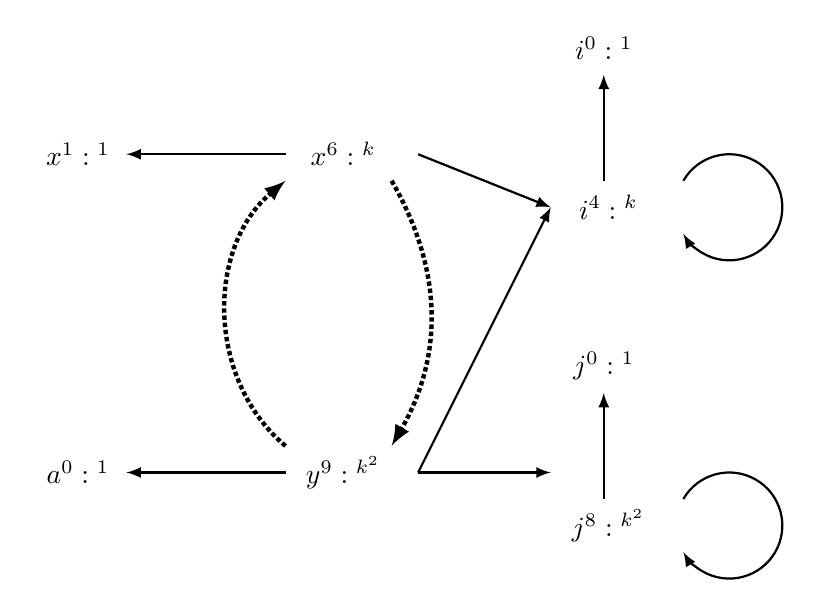
\begin{tikzpicture}[scale=\textwidth/18cm,samples=200]
      % Variables Initialization
      \draw[] (-5, 1) circle (0pt) node{{ $a^0: {}^1$}};
      \draw[] (-5, 7) circle (0pt) node{{ $x^1: {}^{1}$}};
      % Variables Inside the Loop
      \draw[] (0, 7) circle (0pt) node{{ $x^6: {}^{k}$}};
      \draw[] (0, 1) circle (0pt) node{{ $y^9: {}^{k^2}$}};
      % Counter Variables
      \draw[] (5, 9) circle (0pt) node {{$i^0: {}^{1}$}};
      \draw[] (5, 6) circle (0pt) node {{ $i^4: {}^{k}$}};
      \draw[] (5, 3) circle (0pt) node {{$j^0: {}^{1}$}};
      \draw[] (5, 0) circle (0pt) node {{ $j^8: {}^{k^2}$}};
      % Value Dependency Edges:
      \draw[ thick, -latex] (5, 6.5)  --       (5, 8.5) ;
      \draw[ thick, -latex] (5, 0.5)  --       (5, 2.5) ;
      % Value Dependency Edges on Initial Values:
      \draw[ thick, -latex,] (-1, 1)  -- (-4, 1) ;
      \draw[ thick, -latex,] (-1, 7)  -- (-4, 7) ;
      %
      \draw[ ultra thick, -latex, densely dotted,] (-1, 1.5)  to  [out=-220,in=220]  (-1, 6.5);
      % node[left]{\highlight{{$k$}}}
      \draw[ ultra thick, -latex, densely dotted,]  (1, 6.5) to  [out=-60,in=60] (1, 1.5) ;
      % node[right]{\highlight{{$k$}}}
      % Control Dependency
      \draw[ thick, -latex, ] (6.5, 6.5) arc (150:-150:1);
      \draw[ thick, -latex, ] (6.5, 0.5) arc (150:-150:1);
      \draw[ thick,-latex] (1.5, 7)  -- (4, 6) ;
      \draw[ thick,-latex] (1.5, 1)  -- (4, 6) ;
      \draw[ thick,-latex] (1.5, 1)  -- (4, 1) ;
   \end{tikzpicture}
   \caption{}
      \end{centering}
      \end{subfigure}
    }
     \caption{(a) Nested While Loop Example, (b) Execution-Based Dependency Graph, (c) The Static Program-Based Dependency graph.}
    \label{fig:heapcost_example.tex}
    \vspace{-0.5cm}
    \end{figure}
  \end{example}

% As shown in the Example~\ref{ex:heapcost} above, the heap resource consumption during the program 
% execution is accumulating in the same way as the program's adaptivity. 
% Specifically, in the line: 6 and the line : 9
% the list assigned to $x$ and $y$ is re-written instead of accumulated.
% So the heap consumption in the loop isn't accumulated recursively, which is 
% the same as the case where the adaptivity isn't accumulated because of non-dependency between variables.
% In other words, these operations in the above cases imply implicit cost decreases 
% which are all considered as increases in the traditional resource analysis 
% method.

% Following the same system structure as $\THESYSTEM$,
% by modifying the restriction on the finite walk, compute different resource costs for the program.

